% --------------------------------------------------------------
% This is all preamble stuff that you don't have to worry about.
% Head down to where it says "Start here"
% --------------------------------------------------------------
 

\pdfminorversion=7 
\PassOptionsToPackage{dvipdfmx}{graphicx}
\documentclass{beamer}
\usepackage[english]{babel} 
\usepackage[utf8]{inputenc} 
\usepackage{graphicx}
\usetheme{Madrid}
\usecolortheme{whale}

\AtBeginSection[]
{
  \begin{frame}
    \frametitle{Table of Contents}
    \tableofcontents[currentsection]
  \end{frame}
}

\title{Intro to AI and ML}
\subtitle{Matrix Project}
\author{Anjani Kumar\texorpdfstring{\\ Tungadri Mandal}{}} 
\begin{document}
 
% --------------------------------------------------------------
%                         Start here
% --------------------------------------------------------------

\frame{\titlepage}

\begin{frame}
\frametitle{Table of Contents}
\tableofcontents
\end{frame}

\section{Problem Statement}
\begin{frame}
\frametitle{Problem Statement }
Original Question\\
The equation of the circle which is the mirror image of the circle\\
\begin{equation}
    \boldsymbol{{x^2}+{y^2}-2x=0}
\end{equation}
about the line\\
\begin{equation}
    \boldsymbol{y=3-x}
\end{equation}
\end{frame}

\begin{frame}
\frametitle{Problem Statement }
Matrix Form\\
Find the equation of the circle, which is the
mirror image of the circle
% 	Y = 1000 - \frac{600}{4} \times (X-2)
\begin{equation}
    \boldsymbol{x^Tx} - (2\hspace{5mm} 0)\boldsymbol{x} = 0
\end{equation}
in the line 
\begin{equation}
    (1\hspace{5mm} 1)\boldsymbol{x} = 3
\end{equation}
\end{frame}

\section{Desired Answer}
\begin{frame}{Desired Answer}
% An image of the given circle, line and it's mirror image attached
\begin{figure}[h]
\centering
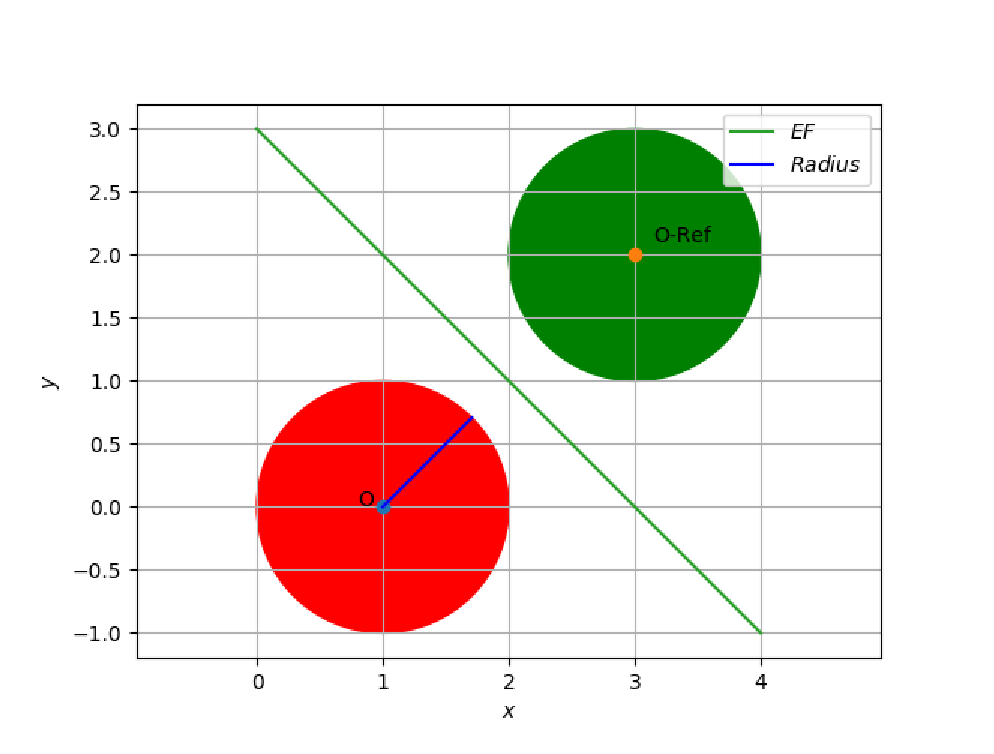
\includegraphics[scale=0.54]{figs/circles.eps}
\caption{Reflection of circle about a line}
\label{etiqueta}
\end{figure}
\end{frame}

\section{Solution}
\begin{frame}{Solution}
\begin{solution}
Let $\boldsymbol{c}$ be the center and r be the radius of the circle respectively.
\begin{equation}
    \Vert\left(\boldsymbol{x - c}) \right\Vert^2 = r^2
\end{equation}
\begin{equation}
    \Rightarrow \boldsymbol{(x-c)^T(x-c)} = r^2
\end{equation}
\begin{equation}
    \Rightarrow \boldsymbol{x^Tx - 2c^Tx} = r^2 - \boldsymbol{c^Tc}
\end{equation}
Comparing with eqn(1),
\begin{align}
    \boldsymbol{c} &= \begin{bmatrix}
           1 \\
           0 \\
         \end{bmatrix}
\end{align}
\begin{equation}
    r^2 - \boldsymbol{c^Tc} = 0 \Rightarrow r = 1
\end{equation}  
\end{solution}
\end{frame}

\begin{frame}
\begin{solution}
We have the equation of line as
\begin{equation}
    (1\hspace{5mm} 1)\boldsymbol{x} = 3
\end{equation}
this can be written in the form
\begin{equation}
    \boldsymbol{Nx = } C
\end{equation}
where N is the normal to the line and C is a constant.\\
Comparing with eqn(8),\\
\begin{align}
    \boldsymbol{N} &= \begin{bmatrix}
           1 \\
           1 \\
         \end{bmatrix}
\end{align}

Intersection of line (passing through center $\boldsymbol{c}$ and $\boldsymbol{c + 0.1N}$) with the given line gives the foot of perpendicular on the given line from $\boldsymbol{c}$.\\
\end{solution}
\end{frame}

\begin{frame}
\begin{solution}
Let $\boldsymbol{f}$ and $\boldsymbol{c'}$ be the foot of perpendicular and image of center respectively.\\
Then we have 
\begin{equation}
    \frac{\boldsymbol{c+c'}}{2} = \boldsymbol{f}
\end{equation}
\begin{equation}
    \Rightarrow \boldsymbol{c' = 2f + c}
\end{equation}
Since the radius remains same after reflection, we have equation of reflected circle as 
\begin{equation}
    \boldsymbol{x^Tx - 2c'^Tx} = r^2 - \boldsymbol{c'^Tc'}
\end{equation}
\end{solution}
\end{frame}
\begin{frame}{Conclusion}
\begin{block}{Conclusion}
So,the reflected circle is\\
\begin{equation}
    \boldsymbol{x^Tx - 2c'^Tx} = r^2 - \boldsymbol{c'^Tc'}
\end{equation}
\end{block}
\end{frame}

\section{ Walkthrough of the code }

\begin{frame}{Walkthrough of the code(Functions)}
\textbf{function norm\_vec(AB)}\hfill //returns the normal vector of line AB.\\
\textbf{function mid\_pt(B,C)}\hfill //calculates the mid point of two given points.\\
\textbf{function line\_intersect\_normal\_form(N,P)}\hfill //creates a line from normal form.\\
\textbf{function line\_intersect\_normal\_form(N,P)}\hfill //returns reflection of a point about a line.\\
\end{frame}

\begin{frame}{Walkthrough of the code(Main Section)}
\textbf{MAIN SECTION}\\
// centre of the circle \\
\textbf{cen=np.matmul(cenM,A.T)} \\

// constant term for the circle \\
\textbf{D=0} \\

// Reflected centre \\
\textbf{refCen=reflection\_normal\_form(B,C,cen)} \\

// Radius of the circle \\
\textbf{radius=(cen[0]**2+cen[1]**2-D)**0.5} \\

// Foot of perpendicular of the center to the line \\
\textbf{E=(cen+refCen)/2} \\
\end{frame}

% --------------------------------------------------------------
%     You don't have to mess with anything below this line.
% --------------------------------------------------------------
 
\end{document}
